\section{Asymmetric Interconnects}
\label{sec:interconnect}

Figure~\ref{fig:symmetric_assymetric}(a) shows a switch connected GPU
with symmetric and static link bandwidth assignment.
Each link is comprised of equal number of uni-directional high-speed
lanes in both directions, collectively comprising a symmetric bi-directional
link. Traditional static design time link capacity assignment is very common and has
several advantages. For example, only one type of I/O circuitry
(egress drivers or ingress receivers) along with only one type of control logic
need to be implemented at each on-chip link interface. Moreover, the multi-socket
switches result in simpler designs that can easily support a statically provisioned
bandwidth requirements. On the other hand, multi-socket link bandwidth utilization can have
a large impact on overall system performance. Static partitioning of bandwidth,
when application needs are dynamic, can leave performance on the table.
Because I/O bandwidth is a limited and expensive system resource, NUMA-aware
interconnects designs must look for innovations that can keep wire and I/O
utilization high. 

In multi-socket NUMA GPU systems, we observe that many applications have 
different utilization of egress and ingress channels on both a per GPU-socket basis
and during different phases of execution. For example,
Figure~\ref{fig:link-motivation} shows a link utilization snapshot over time for
\texttt{HPC-HPGMG-UVM} running on a SW locality optimized 4-socket NUMA GPU. 
Vertical dotted black lines represent
kernel invocations that are split across the 4 GPU-sockets. We can see that 
several small kernels have
negligible interconnect utilization. However, for the later
larger kernels, GPU0 and GPU2 fully saturate their ingress links,
while GPU1 and GPU3 fully saturate their egress links. At the same time GPU0 
and GPU2, and GPU1 and GPU3 are underutilizing their egress and ingress links respectively.

\begin{figure}[t]
    \centering
    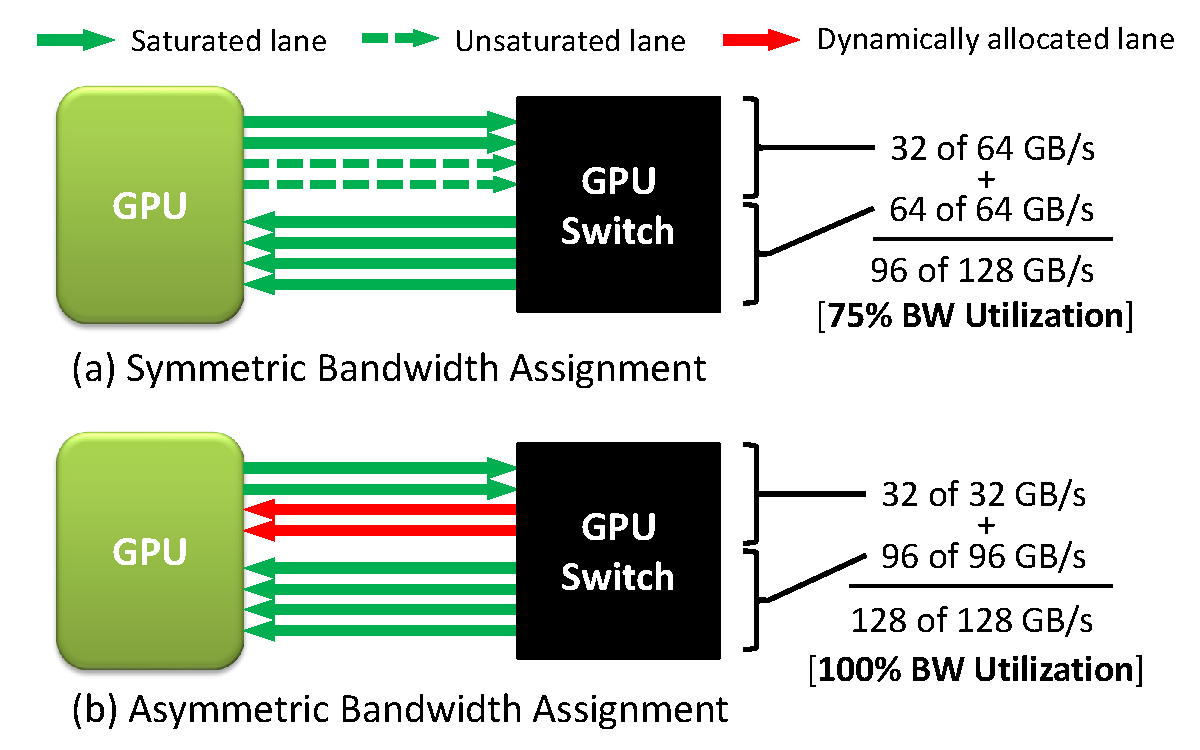
\includegraphics[width=1.0\columnwidth]{figures/link_assignment.pdf}
    \caption{Example of dynamic link assignment to improve interconnect efficiency.}
    \label{fig:symmetric_assymetric}
    \vspace{-.2in}
\end{figure}

In many workloads we observe one common
scenario, in which all CTAs writing to the same memory range at the end of a
kernel (i.e. parallel reductions, data gathering). For CTAs running on one of the
sockets, GPU0 for example, these memory references are local and do not
produce any traffic on the inter-socket interconnections. However CTAs dispatched
to other GPUs must issue remote memory writes, saturating their egress links while
ingress links remain underutilized, but causing ingress traffic on GPU0. 
Such communication patterns typically utilize only
50\% of available interconnect bandwidth. In these cases, dynamically increasing the 
number of ingress lanes for GPU0
(by turning around direction of egress lanes) and switching the direction of
ingress lanes for GPUs 1--3, can substantially improve the achievable interconnect
bandwidth. Motivated by these findings, we propose to dynamically control multi-socket
link bandwidth assignments on a per-GPU basis resulting in
dynamic asymmetric link capacity assignments as shown in
Figure~\ref{fig:symmetric_assymetric}(b).  

To evaluate this proposal we model point-to-point links containing multiple 
lanes, similarly to NVLink~\cite{pascal-tesla-wp}. In these links, 8 
lanes with 8GB/s capacity per lane yield an aggregate bandwidth of 64GB/s in 
each direction. We propose replacing uni-directional lanes with bi-directional 
lanes to which we apply an adaptive link bandwidth allocation mechanism that 
works as following. For each link in the system, at kernel launch the links are 
always reconfigured to contain symmetric link bandwidth with 4 lanes per 
direction. During kernel execution the link load balancer periodically samples 
the saturation status of each link. If the lanes in one direction are not 
saturated, while the lanes in the opposite direction are 99\% saturated, the 
link load balancer reconfigures and reverses the direction of one of the 
unsaturated lanes after quiescing all packets on that lane. 

This sample and 
reconfigure process stops only when directional utilization is not 
oversubscribed or all but one lane is configured in a single direction. If 
both ingress and egress links are found to be saturated and in an asymmetric 
configuration, links are then reconfigured back towards a symmetric configuration 
to encourage global bandwidth equalization. While this process may sound 
complex, the circuitry for dynamically turning high speed single ended links 
around in a short number of cycles already is in use by modern high bandwidth 
memory interfaces such as GDDR; where the same set of wires is used for both memory reads 
and writes~\cite{hynixgddr51Gb}.

\subsection{Results and Discussion} 

There are two important parameters that will affect the performance of
our proposed mechanism (i)
\texttt{SampleTime}: The frequency at which the scheme samples for a possible
reconfiguration and (ii) \texttt{SwitchTime}: The cost of turning the
direction of an individual lane. Figure~\ref{fig:sampletime} shows the 
performance improvement, with
respect to our SW locality optimized GPU by exploring different values of the
\texttt{SampleTime} indicated by green bars and assuming a \texttt{SwitchTime}
of 100 cycles. The red bars in Figure~\ref{fig:sampletime} provide an
upper-bound of performance speedups when doubling the available interconnect
bandwidth to 256GB/s. For workloads on the right of the figure, doubling the link
bandwidth has little effect, thus dynamic link policy will also show little
improvement due to low GPU--GPU interconnect bandwidth needs.
On the left side, we can see that for some
applications, where improved interconnect bandwidth has a large effect,
dynamic lane switching can improve application performance by as much as 80\%.
For some benchmarks like \texttt{Rodinia-Euler-3D}, \texttt{HPC-AMG}, and 
\texttt{HPC-Lulesh}, doubling the link bandwidth provides 2$\times$ 
speedup, while our proposed dynamic link assignment mechanism is not 
able to significantly improve performance. Those are the workloads 
that saturate both link directions, so there is no opportunity to 
provide additional bandwidth by turning links around.

Using a moderate 5K cycle sample time, dynamic link policy can improve performance
by 14\% on average over static bandwidth partitioning. If the link load
balancer samples too infrequently application dynamics can be missed
and performance improvement is reduced. However if the link is turned around
too frequently, bandwidth is lost due to the overhead of turning the link.
While we have assumed a pessimistic link turn time of 100 cycles, we performed
sensitivity studies that show even if link turn time were increased to 500
cycles, our dynamic policy loses less than 2\% of performance. 
At the same time, using a faster lane switch (10 cycles) does not
significantly improve the performance over a 100 cycle link turn time.
We note that the link
turnaround times of modern high-speed on-board links such as
GDDR5~\cite{hynixgddr51Gb} are about 8ns including both link and internal 
DRAM turn-around latency (which is less than 10 cycles at 1GHz).

\begin{figure}[t]
    \centering
    
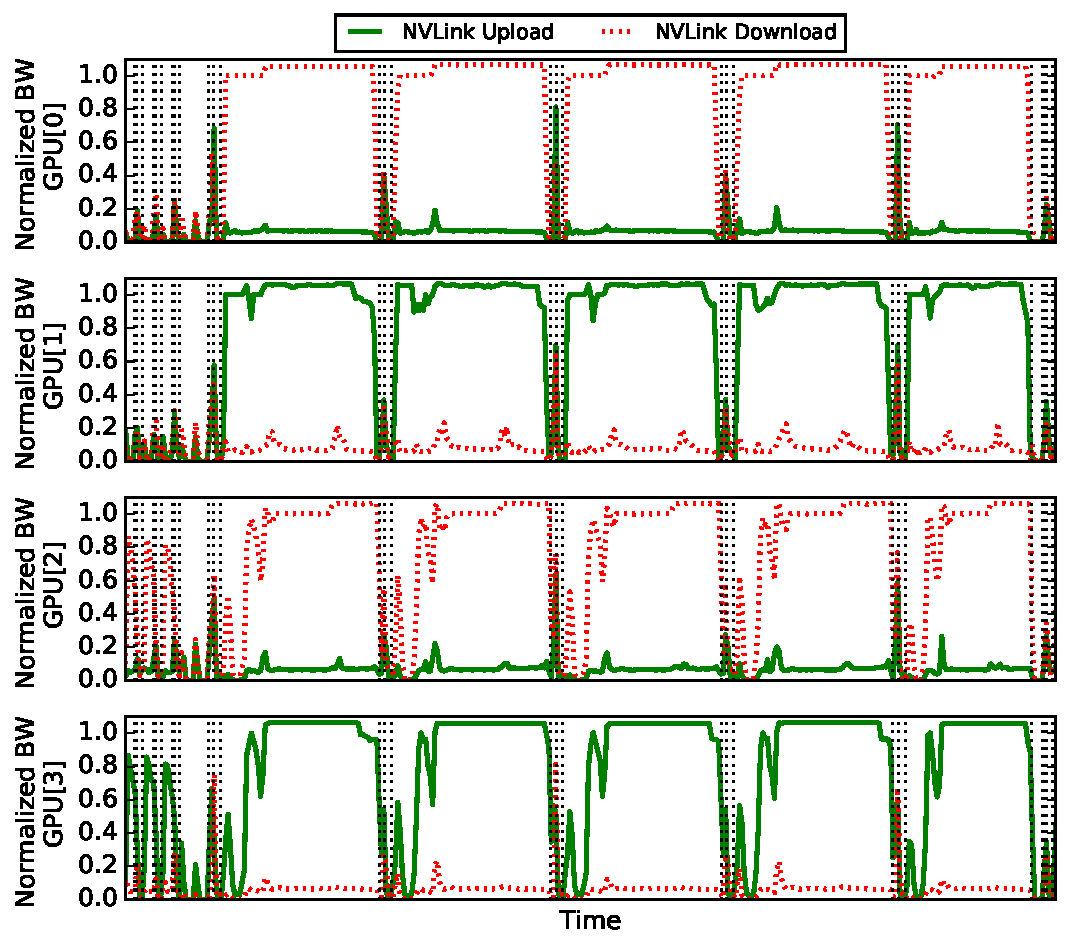
\includegraphics[width=1.0\columnwidth]{figures/bw_profile_HPGMG_UVM_base.pdf}
    \caption{Normalized link bandwidth profile for \texttt{HPC-HPGMG-UVM} 
showing asymmetric link utilization between GPUs and within a GPU. Vertical black 
dotted lines indicate kernel launch events.}
    \label{fig:link-motivation}
    \vspace{-.2in}
\end{figure}

\begin{figure*}[tp]
    \centering
    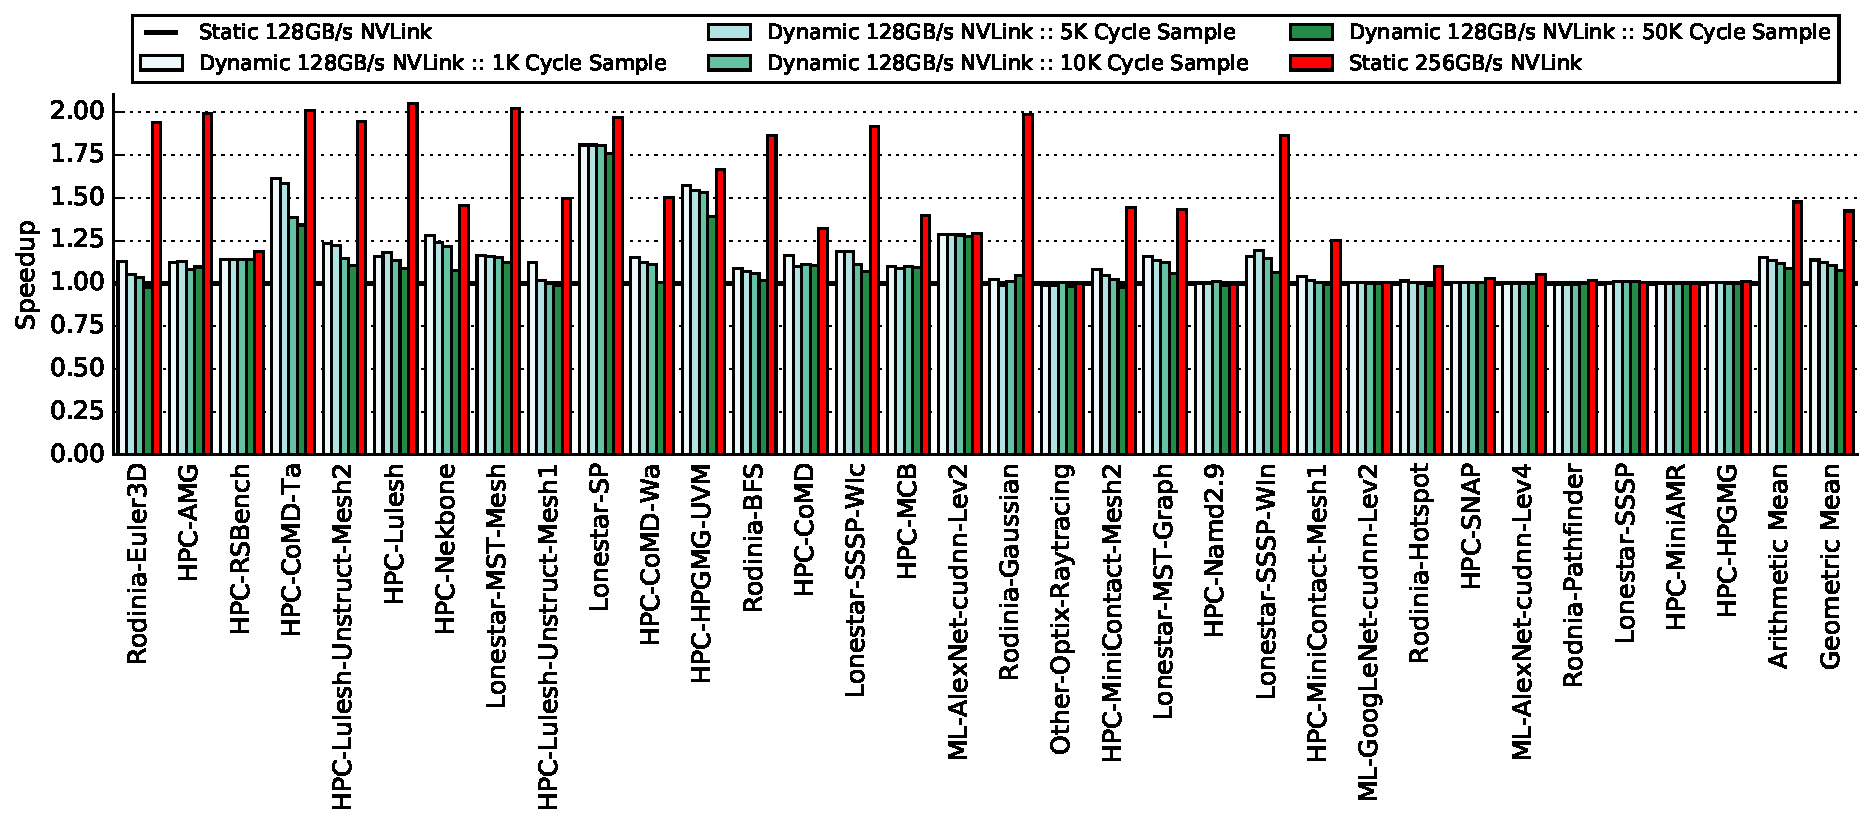
\includegraphics[width=1.0\textwidth]{figures/plot_nvlink_sample_time.pdf}
    \caption{Relative speedup of the dynamic link adaptivity with respect to
	the baseline architecture by varying sample time and assuming switch 
time of
	100 cycles. In red, speedup achievable by doubling link 
bandwidth.}
    \label{fig:sampletime}
    \vspace{-.2in}
\end{figure*}

Our results demonstrate that asymmetric link bandwidth
allocation can be very attractive when inter-socket interconnect bandwidth is constrained 
by the number of on-PCB wires (and thus total link bandwidth).
The primary drawback of this solution is that both types of interface circuitry (TX and RX)
and logic need to be implemented for each lane in both the GPU and switch interfaces.
We conducted an analysis of the potential cost of doubling the amount
of I/O circuitry and logic based on a proprietary state of
the art GPU I/O implementation. Our results show that doubling this interface area
increases total GPU area by less than 1\% while yielding a 12\% improvement in average
interconnect bandwidth which results in a 14\% application performance improvement.  
One additional caveat worth noting is that the proposed asymmetric link
mechanism optimizes link bandwidth in a given direction for each individual
link, while the total switch bandwidth remains constant.
%This means that potential improvement is subject to per-link imbalance and cannot improve
%situations where there is large global bandwidth imbalance occurring.
 

% DO NOT REMOVE, we can use this to compute POWER later 
%from http://teams.nvidia.com/sites/Corporate/ntech/SiteAssets/downloads/2014/NTECH2014_SlideDecks20(presented)/7.1_Osborn.pptx 
%Power: 8 lanes (TX + RX) at 25GT/s ~= 1.5W 
%Area: 8 Lane PHY (8 TX + 8 RX + PLL) ~= 3.3mm^2 
%Physical Data: 7.5pJ/b transferred



